% !TeX root = ../main.tex
\chapter{测量方案设计}\label{ch:principle}

已有的静电力测量方法均具有较大的不确定性。为了得到更准确、可信的测量结果,需解决一些已有方案中的共有问题,并尽可能减小乃至消除测量中的不确定性,设计出新的测量方案。由于除背吹平衡法以外的方案均在原理上就具有较大不确定度(见\ref{sec:priorArt}),此处仅以背吹平衡法作为基础来设计新方案。



\section[背吹法原理分析]{背吹平衡法原理分析}\label{sec:principle-backside}


\subsection{受力分析}\label{sec:principle-backside-force}

\begin{figure}[hbt]
\centering
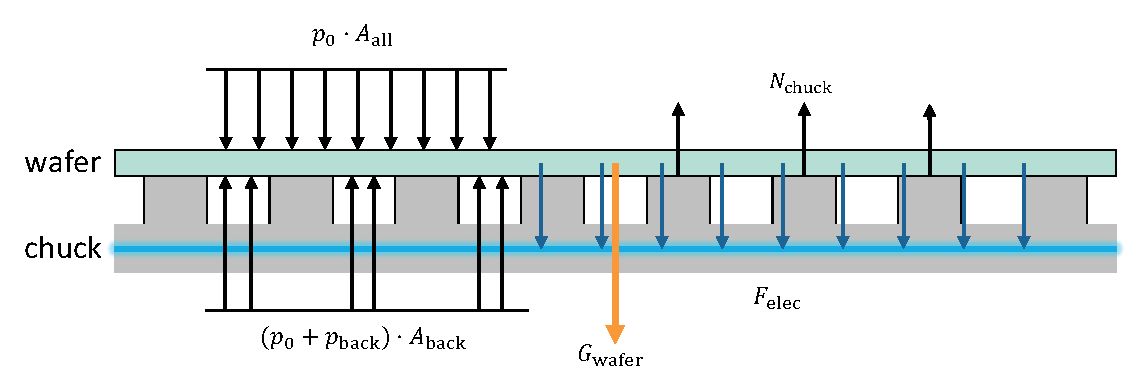
\includegraphics[width=1\linewidth]{principle/force__orig}
\caption[背吹平衡法wafer受力]{背吹平衡法中wafer受力分析图}
\label{fig:principle-backside-force}
\end{figure}

当静电卡盘处于正常工作状态时,wafer牢固吸附在静电卡盘表面,其受力分析如图~\ref{fig:principle-backside-force},有:
\begin{equation}
\label{eq:principle-backside-force}
(p_{0} + p_{\mathrm{back}}) \cdot A_{\mathrm{back}} + N_{\mathrm{chuck}} = p_0 \cdot A_{\mathrm{all}} + G_{\mathrm{wafer}} + F_{\mathrm{elec}}
\end{equation}
其中:
\begin{itemize}
  \item $p_{0}$ : 环境压强(绝对)
  \item $p_{\mathrm{back}}$  : 背吹压强(相对于$p_{0}$)
  \item $A_{\mathrm{back}}$  : wafer背面气压等效作用面积(见\ref{principle-area})
  \item $A_{\mathrm{all}}$   : wafer总面积
  \item $N_{\mathrm{chuck}}$ : 静电卡盘表面向wafer提供的总支持力
  \item $G_{\mathrm{wafer}}$ : wafer总重力
  \item $F_{\mathrm{elec}}$  : wafer所受总静电吸引力
\end{itemize}
当wafer即将脱附时,有 $N_{\mathrm{chuck}} \to 0$ ;此时 \eqref{eq:principle-backside-force} 可近似为:
\begin{equation*}
\label{eq:principle-backside-force'}
(p_{0} + p_{\mathrm{back}}) \cdot A_{\mathrm{back}} = p_0 \cdot A_{\mathrm{all}} + G_{\mathrm{wafer}} + F_{\mathrm{elec}}
\end{equation*}
即:
\begin{equation}
\label{eq:principle-backside-force''}
F_{\mathrm{elec}} = (p_{0} + p_{\mathrm{back}}) \cdot A_{\mathrm{back}} - p_0 \cdot A_{\mathrm{all}} - G_{\mathrm{wafer}}
\end{equation}


\subsection{脱附条件}\label{sec:principle-backside-dechuck}

背吹平衡法需要\emph{制造}并\emph{检测}wafer即将脱附至完全脱附的状态,从而间接获得静电力大小。制造脱附条件的基本方法是使背吹压力相对于静电吸引力更大,可通过提高气压、降低电压等方式实现(见 \ref{sec:priorArt-backside} )。检测脱附的方法主要是监测wafer在脱附时产生变化的物理量,如位移/挠度、电极回路电流、背吹回路压强/流量等。 %TODO:analysis/xref



\section{试验环境}\label{sec:principle-env}

静电卡盘最常见的工作条件是在工艺腔室中,周围环境为真空,有时存在等离子体(单极型静电卡盘必须有等离子体存在才能产生静电吸引力)。已有方案大多选择同样在真空腔室中进行测量,甚至加入等离子体,以复现实际工艺条件。虽然这样可能有助于提高测试结果的准确度,但在真空与等离子体条件下试验存在如下问题:
\begin{itemize}
  \item 需要围绕选定的静电卡盘及试验用到的各种装置搭建专用真空腔室,其设计复杂,加工要求高;一旦更换被测静电卡盘型号,需重新设计腔室及配套系统;这部分的工作量与复杂程度甚至已经逼近刻蚀机的核心部分。
  \item 抽真空需使用真空泵,花费数小时才能达到真空,若需打开腔室进行调整,则需先平衡气压,再改动,再抽真空;费时费力。
  \item 真空下,背吹气体泄漏率较高 %TODO:xref/cite
  ,该流动过程可能对wafer受力产生影响(见\ref{sec:principle-flow}),使数据处理变得复杂。
  \item 有等离子体存在的时候,卡盘上方的空间基本无法放置任何测量装置(否则会遮挡等离子体,或与等离子体互相干扰),这为测量方案的设计带来了相当大的障碍。
\end{itemize}

因此,新方案将首先为大气环境设计,如可能,兼顾在真空条件下使用(原理不变,装置修改尽量小),但不考虑等离子体。



\section{背吹通道流动}\label{sec:principle-flow}

已有背吹平衡方案均假定wafer背面受均匀压强作用,但未论证该假设的合理性 ---  即,背吹通道中存在的稳态流动是否会影响wafer背面受力情况?若有,则测量方案的准确度可能会受到影响。因此,有必要分析wafer背面的流动情况。


\subsection{建立CFD模型}\label{sec:principle-flow-cfd-setup}

为了方便后续仿真工作的开展,此处选择Comsol作为仿真软件;先搭建简化模型,做出基本判断,再根据后续试验需要,进一步添加细节,提高仿真准确度。

\begin{figure}[hbt]
\centering
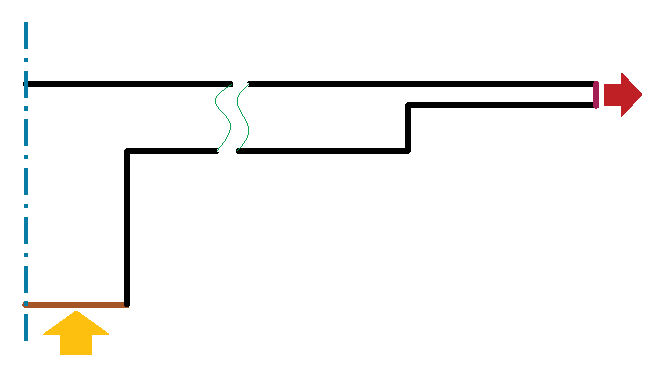
\includegraphics[width=0.72\linewidth]{principle/cfd__setup}
\caption[CFD建模示意]{Wafer背面流动CFD建模示意}
\label{fig:principle-flow-cfd-setup}
\end{figure}

根据静电卡盘几何尺寸,估计流动为充分发展的平板层流,选用\verb|spf|模块求解。几何模型选用\verb|2D Axisymmetric|(即旋转体),流道截面如图~\ref{fig:principle-flow-cfd-setup} 
\footnote{此处流道宽度由陶瓷介电层表面的凸台高度决定,但为了简化分析起见,暂时忽略凸台影响。}
;在正中间设一圆柱形进气口,直径\SI{1}{\mm},固定其压力为\SI{2}{\kPa}表压;在边缘处用均匀圆环形狭缝来等效wafer与陶瓷介电层的接触密封,外侧设为出口,固定为大气压。

由于对实际接触密封情况不是很了解,设定参数扫描,求解狭缝宽度为\verb|10^{range(0,-1/2,-1)}[um]|,即1到\SI{0.1}{\micro\meter}对数等间隔时的流动情况。


\subsection{CFD仿真结果}\label{sec:principle-flow-cfd-result}

当狭缝宽度改变时,速度场变化不大,最大速度均出现在进口附近,之后速度迅速衰减至稳定,如图~\ref{fig:principle-flow-cfd-result-vel} 。

%TODO:动量呢?

在入口处对$v_z\ \rho$取面积分,得到质量流量如表\ref{tab:principle-flow-cfd-result-flow}。单位\si[per-mode=symbol]{\mg\per\minute}大致与sccm相当,即质量流量在狭缝宽\SI{1}{\micro\meter}时,仍低于1 sccm;狭缝变窄时,流量得非常快。这说明只要密封处的实际表面粗糙度足够低,接触足够紧密,则气体泄漏几乎可忽略不计;若安装流量计,则应选取较小量程的型号(一般为10 sccm)。

沿模型上边界(即wafer下表面)绘制压强 -- 半径曲线,如图~\ref{fig:principle-flow-cfd-result-pressure} ,发现在流道中段压降满足$\Delta p \propto \log{r}$。 %TODO:derive by hand
当狭缝宽\SI{1}{\micro\meter}时,在中段存在明显压降(约\SI{0.6}{\kPa}),显然\textbf{不能忽略};但当狭缝更窄时,压降迅速衰减,当狭缝宽\SI{0.3}{\micro\meter}时已可忽略。当然,这是假定只有卡盘中央有一个气孔的时候的情形,而实际的静电卡盘为了控制温度分布均匀,在整个表面多处分布气孔,可使压强分布更均匀。即便如此,在处理实验数据时,应小心验证压强分布(可进一步构建三维流道模型以得到更准确的仿真数据),不能直接认为wafer受均匀气压作用。

\begin{table*}[hbp]
\centering
\caption[CFD结果:质量流量]{CFD仿真结果:进口处质量流量}
\label{tab:principle-flow-cfd-result-flow}
\begin{tabular}{SS}
  \toprule[1.5pt]
  狭缝宽度/\si{\mm}  &  质量流量/\si{\mg\per\minute}  \\
  \midrule[1pt]
  \num{1.000}  &  \num{2.183e-1}  \\
  \num{0.316}  &  \num{9.628e-3}  \\
  \num{0.100}  &  \num{3.079e-4}  \\
  \bottomrule[1.5pt]
\end{tabular}
\end{table*}

\begin{figure}[hbp]
\centering
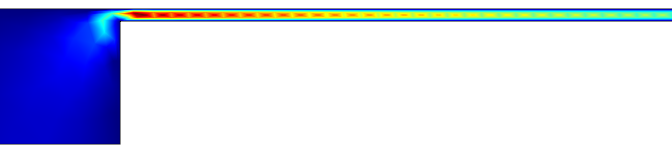
\includegraphics[width=0.72\linewidth]{principle/cfd__vel.png}
\caption[CFD结果:速度场]{CFD仿真结果:进口附近速度场}
\label{fig:principle-flow-cfd-result-vel}
\end{figure}

\begin{figure}[hbp]
\centering
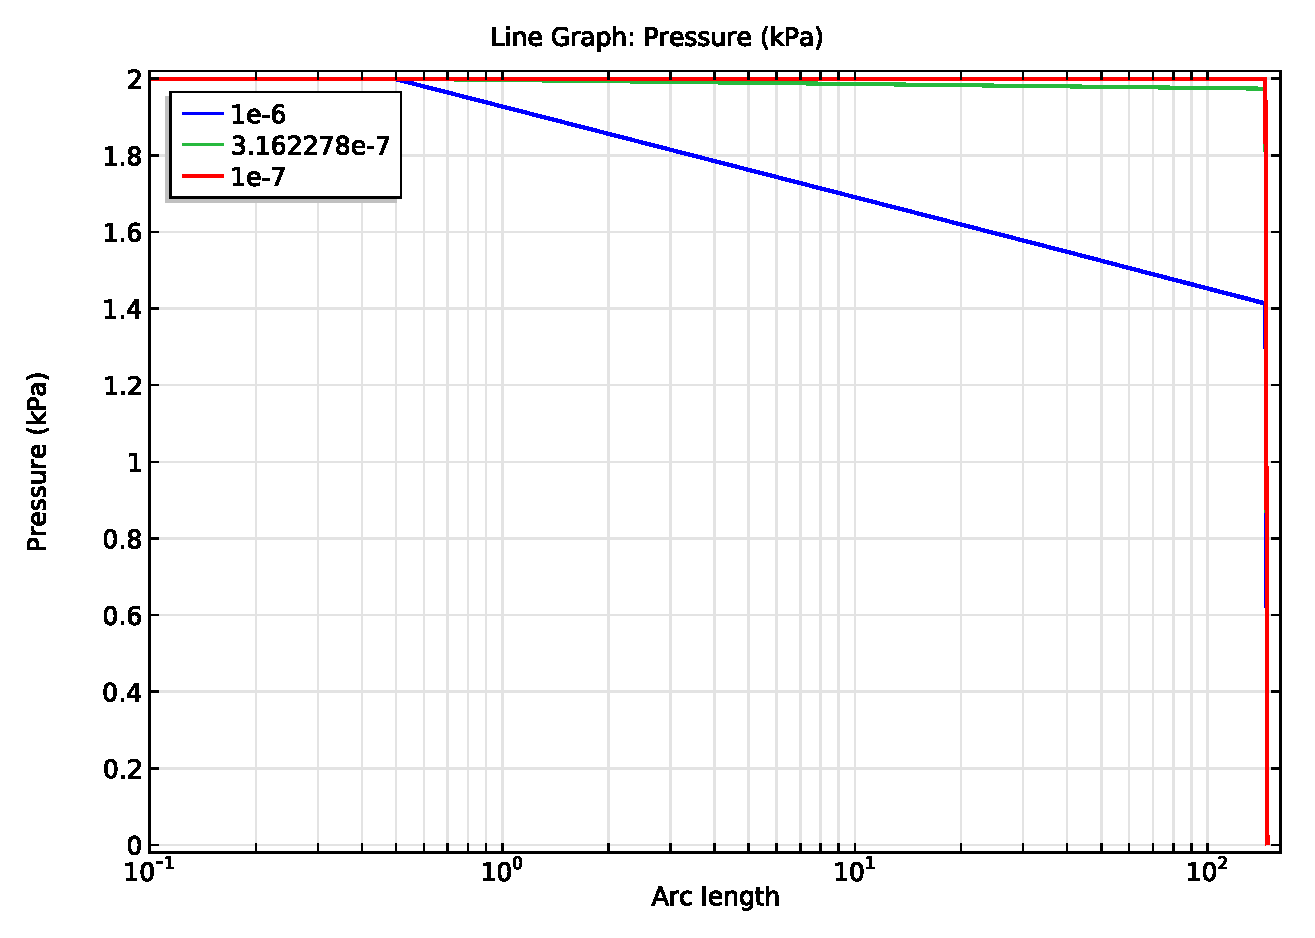
\includegraphics[width=1\linewidth]{principle/cfd__pressure}
\caption[CFD结果:压力分布]{CFD仿真结果:压力沿径向分布}
\label{fig:principle-flow-cfd-result-pressure}
\end{figure}

\clearpage



\section{间隙与部分脱附}\label{principle-gap}

已有脱附试验中(不限于背吹法)另一个共有问题:当\textbf{检测}到脱附时,wafer实际已部分脱附,即脱附是一连续变化的过程  %TODO:cite 曹明路
;此时wafer与卡盘的间隙大于未脱附(正常工作)时,而%TODO:xref bg equations
\begin{comment}
根据,
\end{comment}
静电力随着间隙扩大急剧下降,导致测得的静电力一定小于工作状态静电力,即测量存在较大系统误差。如能设法减小该误差,则可提高测量的准确度。

首先,虽然瞬态过程(如wafer突然出现明显脱附等)容易检测,但此时wafer并非处于平衡态(微观上可能已大部分脱附),且各种测量仪器均有不同程度的响应延迟(精度较高的仪器往往延迟也更大);这些因素均可产生系统误差。因此,应尽可能维持整个测量系统在准静态条件下。

然后,为了尽可能消除部分脱附的影响,希望能在整个脱附过程中尽可能早地检测到“脱附已开始”这一转折点;若此时间隙未明显扩大,则可认为静电力相对于工作状态偏差不大,系统误差减小。这需要选取合适的脱附特征物理量,并在尽量避免误判的同时,提高检测灵敏度。


\subsection{用微力探头减小间隙影响}\label{principle-gap-ruby}

\begin{figure}[tbhp]
\centering
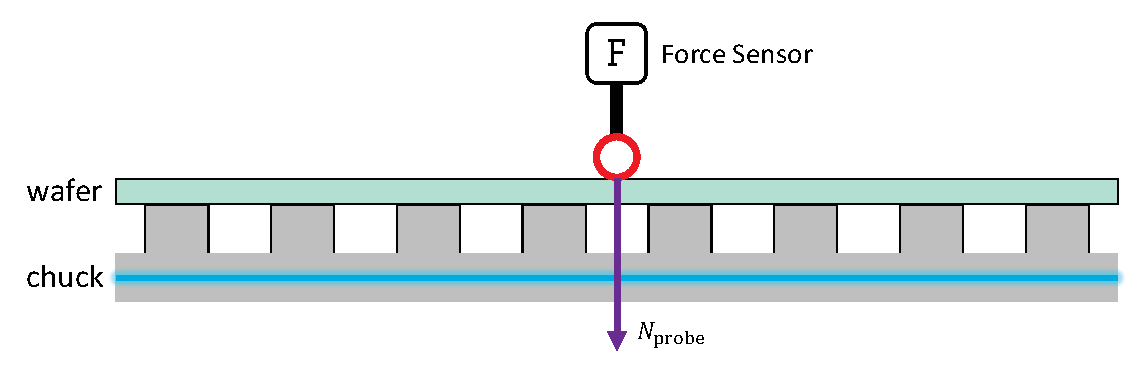
\includegraphics[width=1\linewidth]{principle/gap__ruby__sch}
\caption{微力探头原理示意}
\label{fig:principle-gap-ruby-sch}
\end{figure}

如图~\ref{fig:principle-gap-ruby-sch} ,将一个三坐标测量机标准红宝石探头(图中以红色圆形表示,实际为球面),安装在微力传感器上,即组成一微力探头。将其竖直放置,轻轻接触已吸附的wafer表面。根据受力平衡,微力传感器的读数等于探头向wafer提供的支持力$N_{\mathrm{probe}}$大小。正常工作时,$N_{\mathrm{probe}} \approx 0$。当wafer开始脱附时,卡盘表面不再向wafer提供支持力,即$N_{\mathrm{chuck}} \to 0$,而逐渐转由探头向wafer提供支持力,即$N_{\mathrm{probe}}$逐渐增加。由于力传感器自身具有一定弹性,在此期间容许wafer有一定的挠度,但由于$N_{\mathrm{probe}}$绝对数值较小,可以保证wafer至少在与探头接触的一点处,与卡盘的间隙在一确定范围内,且该范围由传感器参数决定。这样即可较早判定“开始脱附”,并控制此时wafer与卡盘的间隙。

%TODO:introduce F-p curve schematic (or later?)



\section{压强等效作用面积}\label{principle-area}

气压平衡法中,另一个不确定度的来源是wafer背面 气压等效作用面积,即\eqref{eq:principle-backside-force}中的$A_{\mathrm{back}}$。
%TODO:cite nagoya
由于陶瓷介电层上的凸台高度较低(约\SI{10}{\micro\meter})与wafer背面接触情况不明,尚不能直接断言$A_{\mathrm{back}}$等于wafer背面所有未与陶瓷层凸台/边缘接触部分的面积。由于此处无法用普通CFD求解,需要设计额外的标定步骤,测出$A_{\mathrm{back}}$数值。


\subsection{自重平衡法}\label{sec:principle-area-gravity}

\begin{figure}[tbhp]
\centering
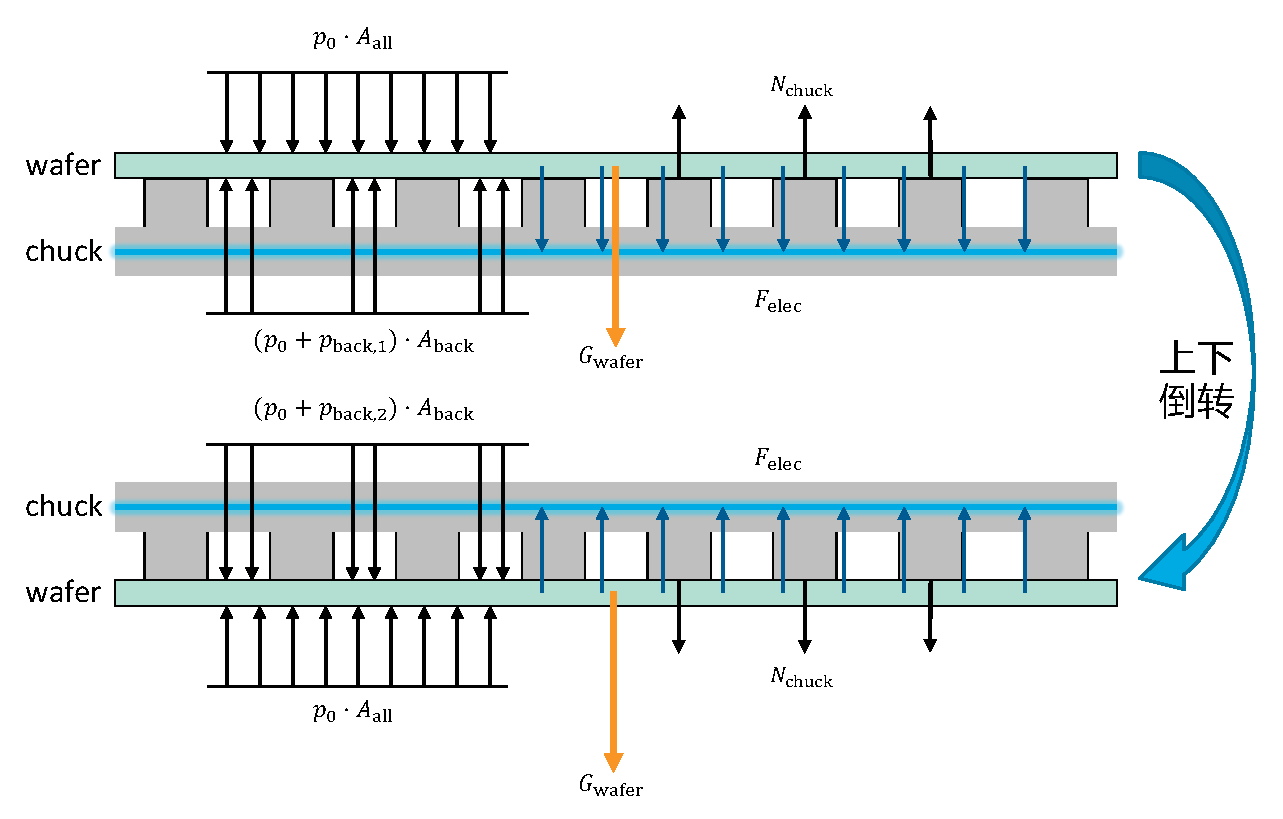
\includegraphics[width=1\linewidth]{principle/area__gravity__sch}
\caption[自重法测等效面积示意]{利用自重平衡法测量压强等效作用面积示意}
\label{fig:principle-area-gravity-sch}
\end{figure}

一种可行的测量方法如图~\ref{fig:principle-area-gravity-sch}。注意到在wafer受力平衡关系中,只有重力的方向是任意的,其他力相对于卡盘坐标系的方向均固定。若将整个系统上下倒转\ang{180},则相当于只有重力的方向发生变化,进而将压强与已知大小的力建立对应关系,得到等效面积大小。

具体方法:分别在试验台正放和倒放两种状态下,加相同电压,完成背吹平衡试验,得到即将脱附时的背吹压强分别为$p_{\mathrm{back},1}$和$p_{\mathrm{back},2}$(可分别多做几组,取平均值,以减小随机误差干扰)。根据受力平衡关系有:
\begin{equation}
\label{eq:principle-area-gravity-orig}
\begin{aligned}
(p_{0} + p_{\mathrm{back},1}) \cdot A_{\mathrm{back}} & = p_0 \cdot A_{\mathrm{all}} + G_{\mathrm{wafer}} + F_{\mathrm{elec}} \\
(p_{0} + p_{\mathrm{back},2}) \cdot A_{\mathrm{back}} & = p_0 \cdot A_{\mathrm{all}} - G_{\mathrm{wafer}} + F_{\mathrm{elec}}
\end{aligned}
\end{equation}
两式相减:
\[
(p_{\mathrm{back},1} - p_{\mathrm{back},2}) \cdot A_{\mathrm{back}} = 2 G_{\mathrm{wafer}}
\]
即:
\begin{equation}
\label{eq:principle-area-gravity-derived}
A_{\mathrm{back}} = \frac{2 G_{\mathrm{wafer}}}{p_{\mathrm{back},1} - p_{\mathrm{back},2}}
\end{equation}
即求得$A_{\mathrm{back}}$数值。需要注意的是,$A_{\mathrm{back}}$可能与所加电压、晶圆材料、厚度等各种参数相关,需改变条件,多次试验,求出$A_{\mathrm{back}}$对各参数的敏感度。




%TODO:summarize what's included in the actual experiment
